\documentclass[a4paper,12pt]{article}
\usepackage{graphicx}
\graphicspath{ {images/} }
\usepackage{multicol}
\setlength{\columnsep}{2cm}
%%% Страница
\usepackage{extsizes} % Возможность сделать 14-й шрифт
\usepackage{geometry} % Простой способ задавать поля
\geometry{top=15mm}
\geometry{bottom=20mm}
\geometry{left=15mm}
\geometry{right=15mm}
\parindent=1cm %Красная строка при абзаце
%
%%% Работа с картинками
\usepackage{graphicx}  % Для вставки рисунков
\graphicspath{{images/}{images2/}}  % папки с картинками
\setlength\fboxsep{3pt} % Отступ рамки \fbox{} от рисунка
\setlength\fboxrule{1pt} % Толщина линий рамки \fbox{}
\usepackage{wrapfig} % Обтекание рисунков текстом
%
%%% Работа с русским языком
\usepackage{cmap} % поиск в PDF
\usepackage{mathtext} % русские буквы в фомулах
\usepackage[T2A]{fontenc} % кодировка
\usepackage[utf8]{inputenc} % кодировка исходного текста
\usepackage[english,russian]{babel} % локализация и переносы

%%% Дополнительная работа с математикой
\usepackage{amsmath,amsfonts,amssymb,amsthm,mathtools} % AMS
\usepackage{icomma} % "Умная" запятая: $0,2$ —- число, $0, 2$ —- перечисление

%% Номера формул
\mathtoolsset{showonlyrefs=true} % Показывать номера только у тех формул, на которые есть \eqref{} в тексте.

%% Шрифты
\usepackage{euscript} % Шрифт Евклид
\usepackage{mathrsfs} % Красивый матшрифт

%% Свои команды
\DeclareMathOperator{\sgn}{\mathop{sgn}}

%% Перенос знаков в формулах (по Львовскому)
\newcommand*{\hm}[1]{#1\nobreak\discretionary{}
	{\hbox{$\mathsurround=0pt #1$}}{}}

\begin{document}

\begin{titlepage}
	\centering
	\vspace{5cm}
	{\scshape\LARGE Московский физико-технический институт \par}
	\vspace{1cm}
	{\scshape\Large Кафедра общей физики \par}
	\vspace{4cm}
	{\scshape\Large Вопрос по выбору \par}
	\vspace{1cm}
	{\huge\bfseries Исследование распространения звуковых волн в разреженном воздухе \par}
	\vspace{1cm}
	\vfill
\begin{flushright}
	{\large выполнили студенты 653 группы ФФКЭ}\par
	\vspace{0.3cm}
	{\LARGE Агафонов Владислав}\par
	\vspace{0.3cm}
	{\LARGE Карпова Татьяна}
\end{flushright}
	

	\vfill

% Bottom of the page
	Долгопрудный, 2017 г.
\end{titlepage}

\part{}
\section{Введение}

Идея исследования пришла к нам после выполнения работы по определению скорости звука (кафедра прикладной механики) и работы по методам получения высокого вакуума (кафедра вакуумной электроники). Нам показалось интересным исследовать распространение звуковых волн в разреженном воздухе (физическом вакууме). \textbf{Гипотеза:} скорость звука с падением давления уменьшается, при малых давлениях звуковые волны не распространяются, так как сходит на нет взаимодействие частиц воздуха между собой.

\section{Зависимость скорости звука от давления в модели реального газа Ван-дер-Ваальса}

Скорость звука в газе определяется по формуле
\begin{equation}
    c = \sqrt{\left ( \frac{\ P}{\ \rho}\right )_S} = \sqrt{\gamma \frac{RT}{\mu}}
\end{equation}

В этой формуле не используется давление. Используя модель газа Ван-дер-Ваальса и работая с частными производными, выведем формулу зависимости скорости звука от давления при постоянной температуре (вывод см. в Приложении 1)

Конечная формула: 

\begin{equation}
c = c_0 \left ( 1 + \frac{2aP}{iRT\mu c^2_0} \right )\left ( 1 + \frac{P}{2RT} \left ( b - \frac{a}{RT} + \frac{2Pab}{(RT)^2} \right ) \right ),
\end{equation}
где $c_0$ - скорость звука по формуле $c = \sqrt{\gamma \frac{RT}{\mu}}$ при определённой фиксированной температуре. 

Построим график зависимости скорости звука от давления на значениях, планируемых для исследования в эксперименте: от 760 торр до 1 торр. Температура 299 К, $c_0 = 346,34 \text{м/с, для воздуха коэффициенты Ван-дер-Ваальса a = 1,3 Н * м}^4 \text{*моль}^{-2} \text{, b = 114,1 см}^3 \text{*моль}^{-1}$.

\begin{figure}[h]
    \centering
    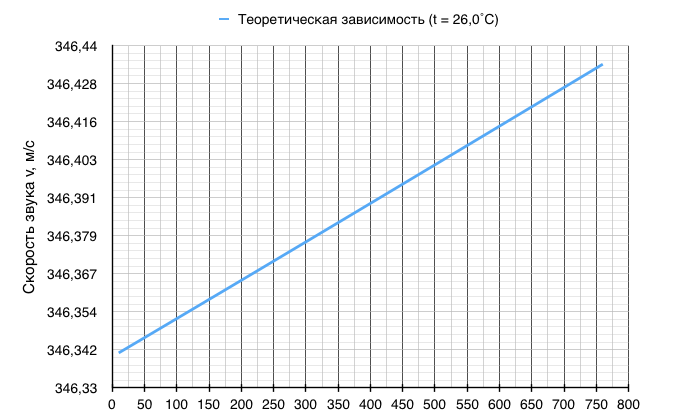
\includegraphics[width=\textwidth]{gr_Th.png}
    \caption{Теоретическая зависимость скорости звука от давления}
    \label{t:final}
\end{figure}

Мы видим, что при уменьшении давления скорость звука изменяется очень незначительно, всего на 0,1 м/с. Такое изменение очень сложно зафиксировать с помощью имеющегося у нас лабораторного оборудования (см. пункт 4). Поэтому в эксперименте будет достаточно проверить то, что скорость звука практически не изменяется, о точном воспроизведении зависимости речи не идёт. \par 

\section{Планирование эксперимента}

\parДля проведения эксперимента мы обратились на кафедру вакуумной электроники, так как там есть оборудование, необходимое для сборки установки: трубы для вакуумной установки, форвакуумный насос, вакуумметр. Неоценимую помощь в сборке вакуумной установки и проведении эксперимента нам оказал преподаватель кафедры Вадим Александрович Буртелов. Были рассмотрены несколько вариантов концепции эксперимента:
\begin{itemize}
    \item Возбуждение колебаний путем пробоя диэлектрика (воздуха) и регистрация времени прохождения звуковой волны по трубе
    \item Метод акустического резонанса: возбуждение резонанса при разных гармониках с помощью пьезокерамики или динамиков мембранного типа
\end{itemize}

Нами был выбран последний вариант как самый надёжный, требующий использования наименьшего количества сложного оборудования. На одном конце трубы планировалось установить динамик, а на другом - приёмник сигналов (по сути, такой же динамик). Измеряя частоты колебаний, необходимые для возбуждения резонанса в трубе на разных гармониках, планировалось определить скорость звука. Резонанс регистрировался на осциллографе, подключенном к приёмнику. Для более точного определения нужной частоты использовался милливольтметр, так как он позволял с большей точностью устанавливать значение амплитуду сигнала. Резонатор присоединён к форвакуумному насосу, к установке присоединён вакуумметр. Установку планировалось откачивать до давления порядка 1 торр. В силу зависимости скорости звука от температуры, к установке был прикреплен термометр.

\section{Сборка экспериментальной установки}

Принципиальная схема установки представлена на рис. 2. \par

\begin{figure}[h]
    \centering
    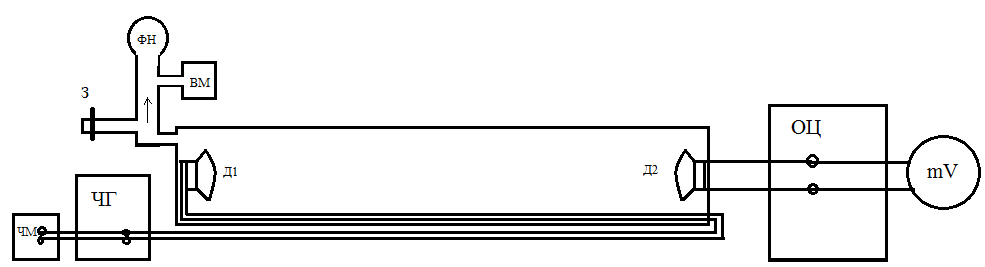
\includegraphics[width=80mm]{setup.png}
    \caption{Принципиальная схема установки}
    \label{setup}
\end{figure}

Используемое оборудование:
\begin{enumerate}
    \item ФН - насос форвакуумный Alcatel Adixen A-120
    \item ВМ - Вакуумметр ёмкостной "Баратрон" (рабочий диапозон давлени1 1 - 1000 торр)
    \item Д1 и Д2 - динамики мембранного типа (передатчик и приёмник соответственно)
    \item ОЦ - осциллограф ламповый С1-70А
    \item mV - Милливольтметр В3-41
    \item ЧГ - частотогенератор ламповый ГЗ-34
    \item ЧМ - частотомер Gwinstek GFC-8010H
    \item Труба\,-\,резонатор длиной $L = 1,1 \text{ м}$
    \item З - зажим на резиновом патрубке
\end{enumerate}

В качестве резонатора была использована вакуумная труба с выходами для проводов - два на осциллограф, два на частотогенератор. Вакуумная установка откачивалась с помощью форвакуумного масляного насоса, установившееся давление регулировалось вручную с помощью зажима на резиновом патрубке.
Фотографии вакуумной установки, крепления проводов и используемых приборов см. в приложении.

\section{Проведение эксперимента}


В основе эксперимента лежит зависимость резонансной частоты от скорости звука:
$$\nu = n \frac{v}{2L}$$,
\begin{equation}
\begin{aligned}
    \nonumber
	\text{где } \nu  &- \text{резонансная частота}\\
	v  &- \text{скорость звука}\\
	L  &- \text{длина трубы - резонатора}\\
\end{aligned}
\end{equation} 

Плавно увеличивая частоту генератора, получим ряд последовательных резонансных значений частоты, отмечая момент резонанса по увеличению амплитуды колебаний на экранах осциллографа (грубо) и милливольтметра(точно). Отметим точки на графике, по оси абцисс откладывая номер гармоники, а по оси ординат соответствующую резонансную частоту. Через полученные точки проведем наилучшую прямую и найдём её коэффициенты, используя метод наименьших квадратов. Погрешности также определяются по МНК. Угловой коэффициент построенной прямой в точности равен $k = \frac{v}{2L}$, где $L$ - длина трубы\,-\,резонатора, a $v$ - скорость звука. Отсюда получим выражение для скорости звука $v = 2Lk$. Повторяемость опытов была проверена при уменьшении частоты. Далее медленно уменьшалась величина натекания воздуха в установку, таким образом создавалось требуемое пониженное давление. После каждого снижения давления требовалось остановить проведение измерений до установления термодинамического равновесия (понижение температуры при изохорном понижении давления). Повторяемость эксперимента также была проверена при увеличении давления. Для вычисления погрешности используем следующую формулу:
$$\sigma_v = \sqrt{\sigma_k^2 + \sigma_L^2}$$

Данные, полученные в ходе опытов, представлены в приложении. Таблица с результатами опытов представлена ниже на рисунке \ref{t:final}. Сравнение теоретических оценок с полученными результатами представлено на рисунке \ref{gr:final}. Интересно, что при давлении 13,2 торр распространение звука подтверждалось колебанием стрелки вольтметра при достижении резонансной частоты, но определить её в заданной точностью не представлялось возможным. К сожалению, чувствительность приборов не позволяла зафиксировать изменение значений амплитуд при меньших давлениях ввиду их малости, поэтому проверить границы применимости используемой модели также не удалось.

\begin{figure}[h]
    \centering
    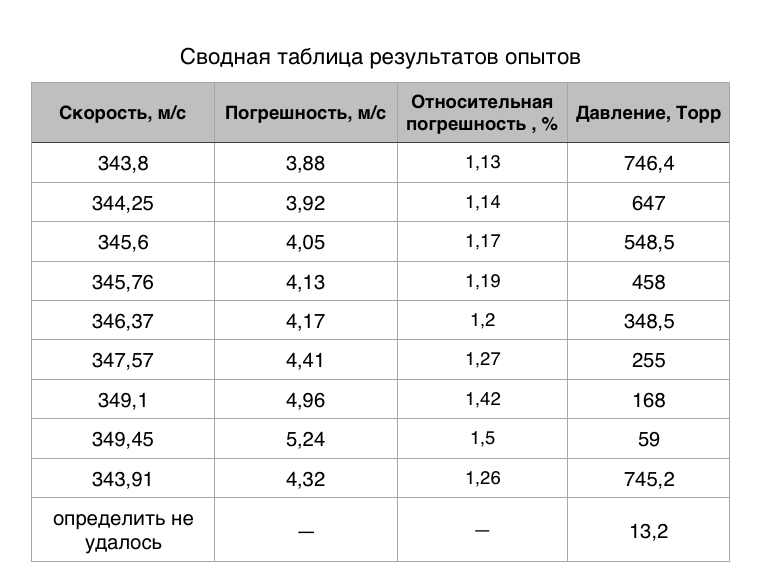
\includegraphics[width=75mm]{t_Final.png}
    \caption{Результаты опытов}
    \label{t:final}
\end{figure}




\begin{figure}[h]
    \centering
    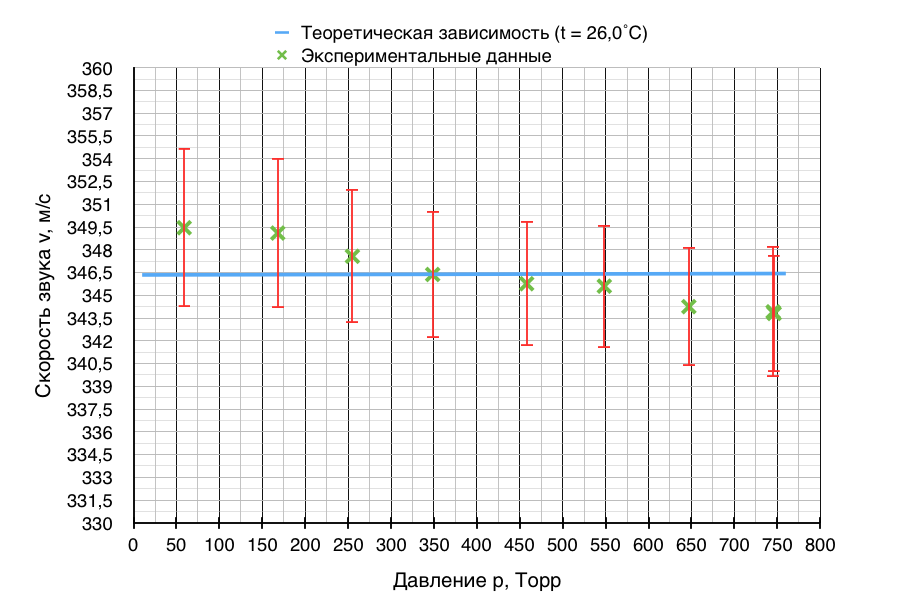
\includegraphics[width=\textwidth]{gr_Final.png}
    \caption{Зависимость скорости звука от давления}
    \label{gr:final}
\end{figure}

\section{Исследование изменения амплитуды}

Как известно, уже в среднем вакууме (длина свободного пробега частицы сравнима с размерами сосуда) звук не распространяется, так как практически отсутствует взаимодействие молекул между собой. В эксперименте мы подтвердили, что с помощью термодинамики нельзя объяснить "исчезновение" скорости звука: сама величина при разрежении газа не изменяется. Поэтому необходимо учитывать взаимодействия на молекулярном уровне. \par 
В нашем опыте в качестве источника и приёмника звука использовался мембранный динамик. Мембрана колеблется и колеблет молекулы воздуха, генерируя звуковые волны. Чем больше плотность газа, с которым взаимодействует мембрана, тем большую энергию она передаёт. Энергия колебаний пропорциональна квадрату их амплитуды. Точно такая же ситуация происходит и с приёмником.  \par 
При уменьшении давления в m раз во столько же раз уменьшится концентрация частиц в резонаторе. Энергия пропорциональна концентрации и также уменьшится в m раз. Энергия пропорциональна квадрату амплитуды - А уменьшится в $\sqrt m$ после выхода из излучателя и во столько же раз на входе в приёмник: А, регистрируемая на осциллографе, также уменьшится в m раз. Эта зависимость имеет очень приближённый характер, и в нашем эксперименте соблюдается лишь на нескольких гармониках. Но тем не менее очевидно, что при уменьшении концентрации молекул в воздухе амплитуда звуковой волны в нём падает. Приведём экспериментально полученные графики зависимости амплитуды принимаемого сигнала от давления в резонаторе. \par

\begin{figure}[h]
    \centering
    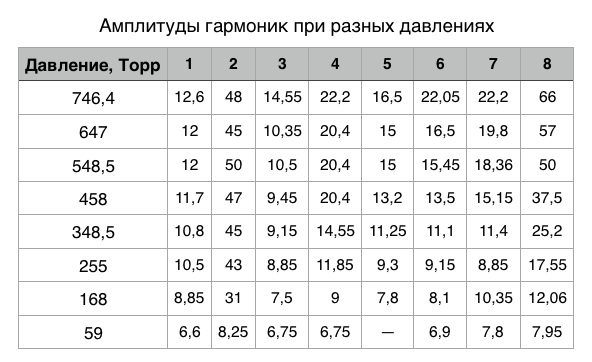
\includegraphics[width=\textwidth]{t_A(p).png}
    \caption{Зависимость скорости звука от давления}
    \label{gr:final}
\end{figure}

\begin{figure}[h]
    \centering
    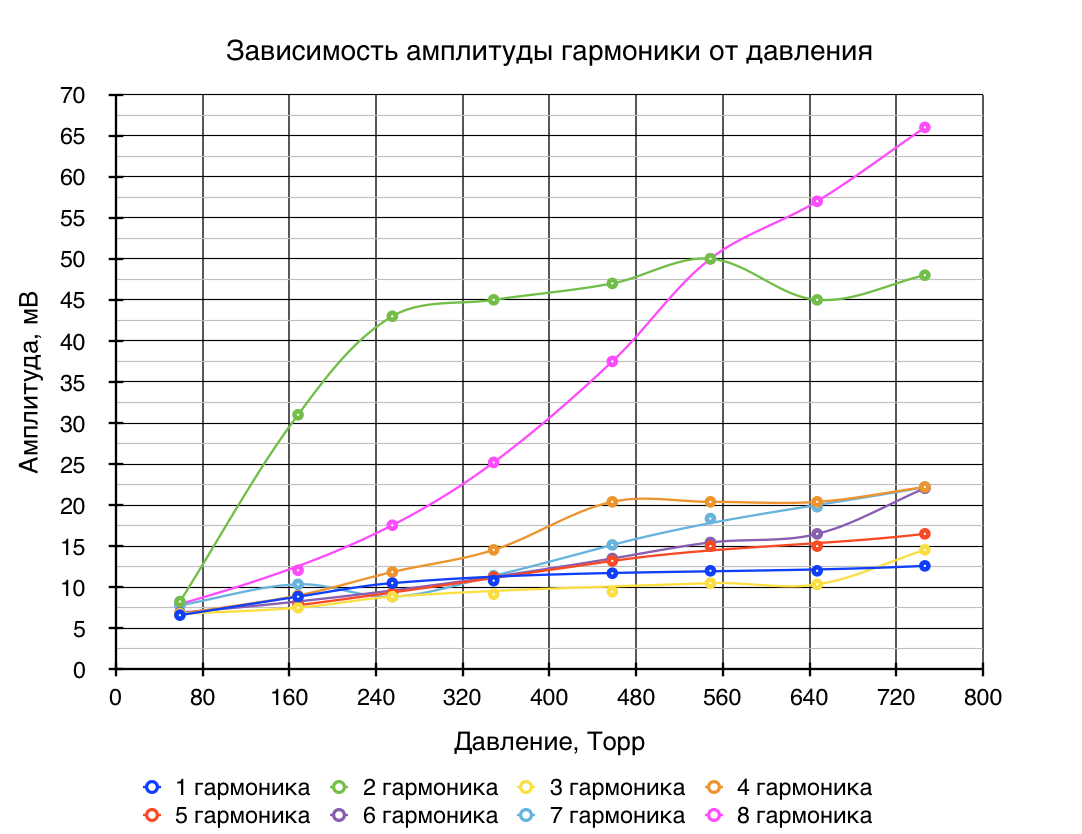
\includegraphics[width=\textwidth]{gr_A(p).png}
    \caption{Зависимость амплитуды звуковой от давления}
    \label{gr:final}
\end{figure}
Возможно, при наличии более совершенного и точного оборудования, зависимость амплитуды от давления газа в резонаторе можно было бы измерить с большей точностью и проверить эмпирическую зависимость, полученную выше.

\clearpage

\section{Вывод}
В качестве логического продолжения данной работы интересно исследовать границы применимости данной модели, когда распространение звука не описывается моделями термодинамики. Также при наличии более точного измерительного оборудования можно провести более точное исследование зависимости амплитуды распространяемой звуковой волны и определить характер зависимости.


\newpage
\clearpage
\part{Приложения}
\setcounter{section}{0}
\section{Данные эксперимента}

\setcounter{figure}{0}
\begin{figure}[h]
	\begin{multicols}{2}
		\hfill
		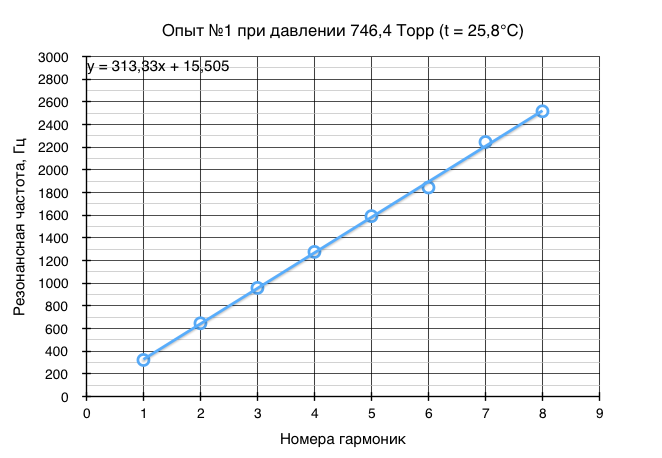
\includegraphics[width=40mm]{gr1.png}
		\hfill
		%\caption{Опыт №1}
		\label{gr1}
		\hfill
		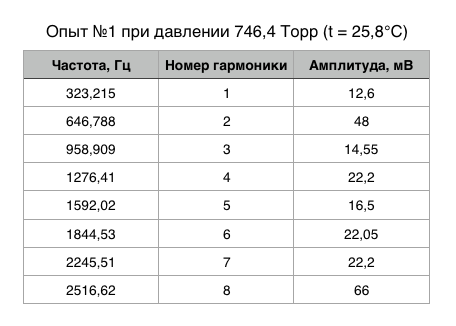
\includegraphics[width=40mm]{t1.png}
		\hfill
		%caption{Опыт №1}
		\label{t1}
	\end{multicols}
\end{figure}
\begin{figure}[h]
	\begin{multicols}{2}
		\hfill
		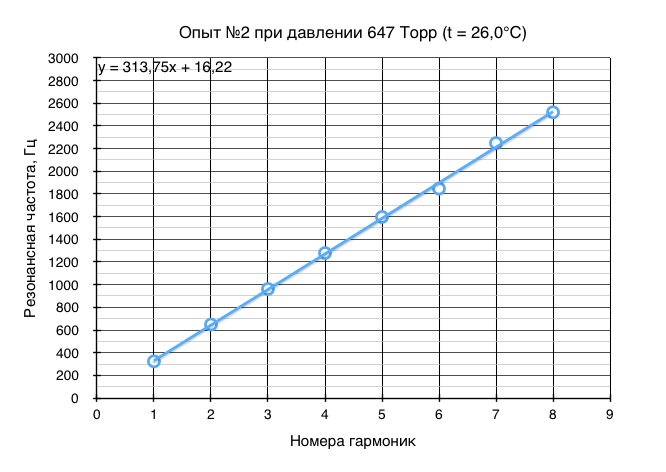
\includegraphics[width=80mm]{gr2.png}
		\hfill
		%\caption{Опыт №1}
		\label{gr2}
		\hfill
		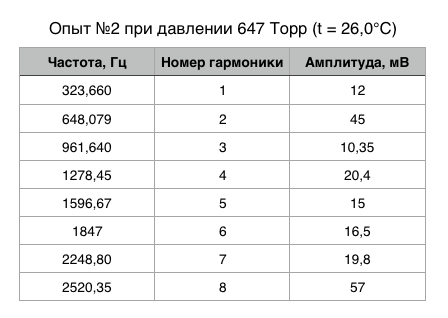
\includegraphics[width=70mm]{t2.png}
		\hfill
		%caption{Опыт №1}
		\label{t2}
	\end{multicols}
\end{figure}
\begin{figure}[h]
	\begin{multicols}{2}
		\hfill
		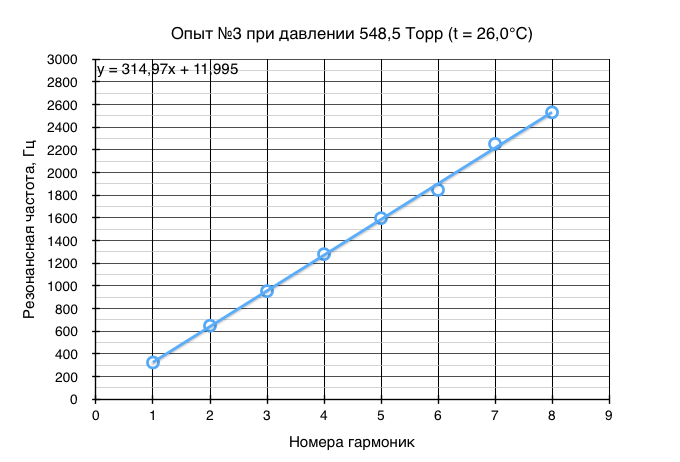
\includegraphics[width=80mm]{gr3.png}
		\hfill
		%\caption{Опыт №1}
		\label{gr3}
		\hfill
		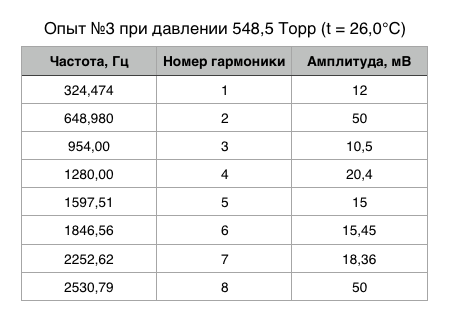
\includegraphics[width=70mm]{t3.png}
		\hfill
		%caption{Опыт №1}
		\label{t3}
	\end{multicols}
\end{figure}
\begin{figure}[h]
	\begin{multicols}{2}
		\hfill
		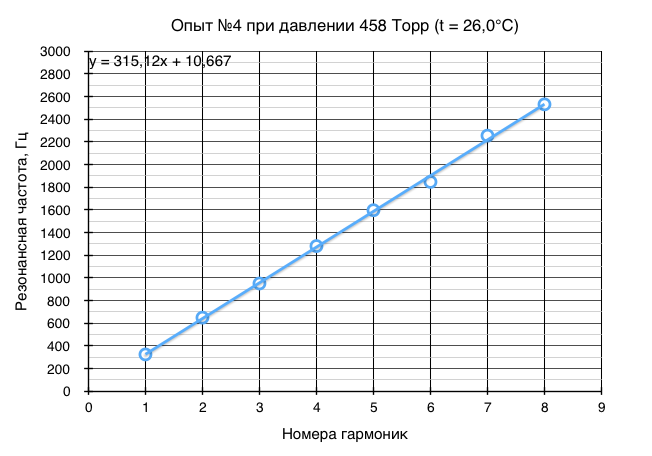
\includegraphics[width=80mm]{gr4.png}
		\hfill
		%\caption{Опыт №1}
		\label{gr4}
		\hfill
		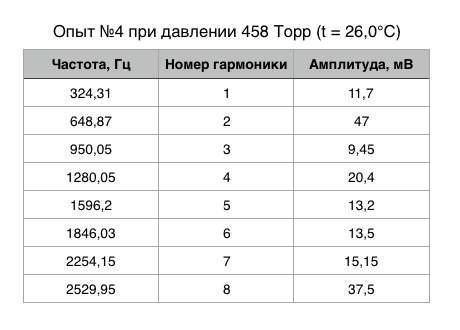
\includegraphics[width=70mm]{t4.png}
		\hfill
		%caption{Опыт №1}
		\label{t4}
	\end{multicols}
\end{figure}
\begin{figure}[h]
	\begin{multicols}{2}
		\hfill
		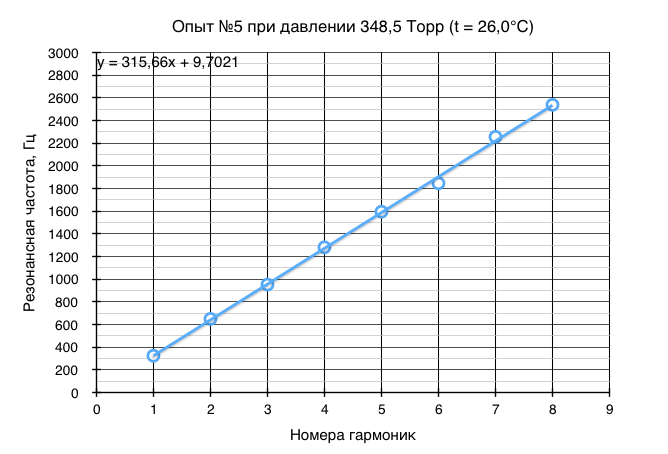
\includegraphics[width=80mm]{gr5.png}
		\hfill
		%\caption{Опыт №1}
		\label{gr5}
		\hfill
		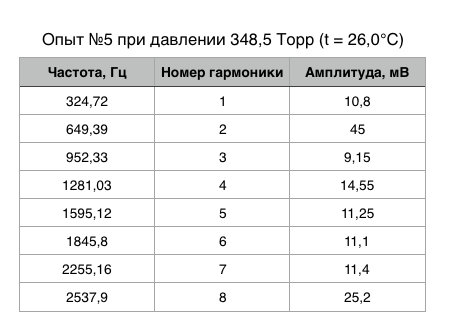
\includegraphics[width=70mm]{t5.png}
		\hfill
		%caption{Опыт №1}
		\label{t5}
	\end{multicols}
\end{figure}
\begin{figure}[h]
	\begin{multicols}{2}
		\hfill
		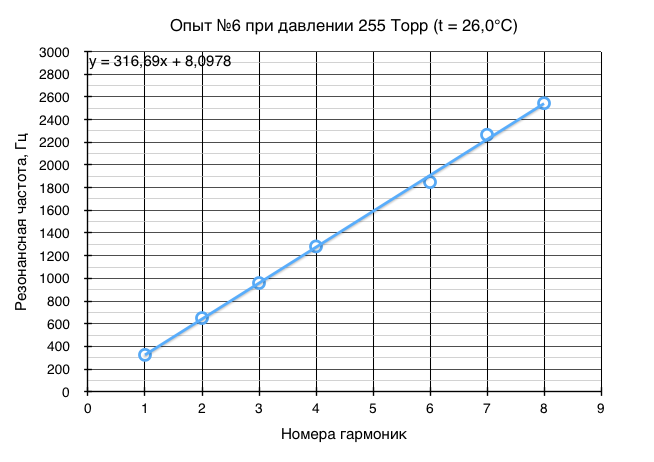
\includegraphics[width=80mm]{gr6.png}
		\hfill
		%\caption{Опыт №1}
		\label{gr6}
		\hfill
		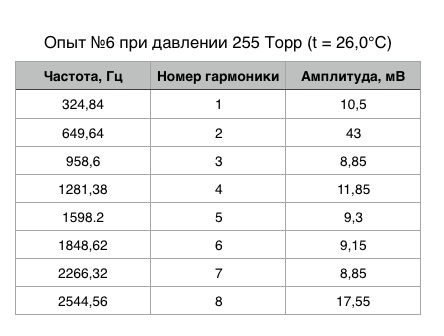
\includegraphics[width=70mm]{t6.png}
		\hfill
		%caption{Опыт №1}
		\label{t6}
	\end{multicols}
\end{figure}
\begin{figure}[h]
	\begin{multicols}{2}
		\hfill
		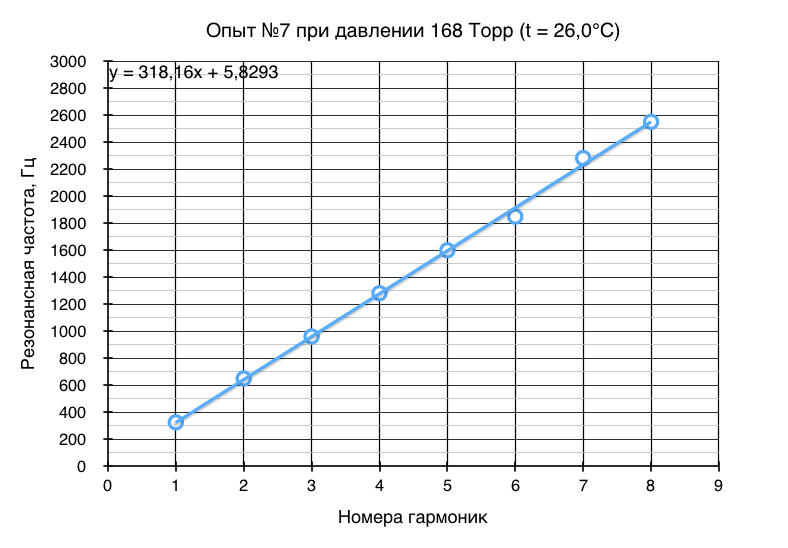
\includegraphics[width=80mm]{gr7.png}
		\hfill
		%\caption{Опыт №1}
		\label{gr7}
		\hfill
		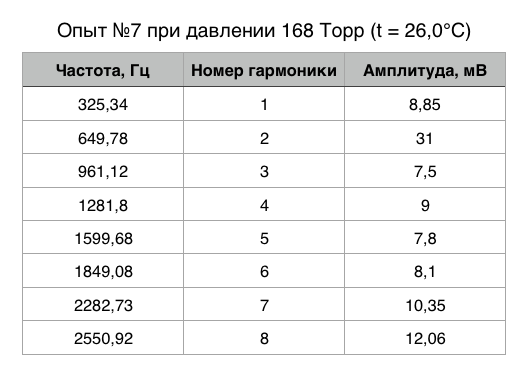
\includegraphics[width=70mm]{t7.png}
		\hfill
		%caption{Опыт №1}
		\label{t7}
	\end{multicols}
\end{figure}
\begin{figure}[h]
	\begin{multicols}{2}
		\hfill
		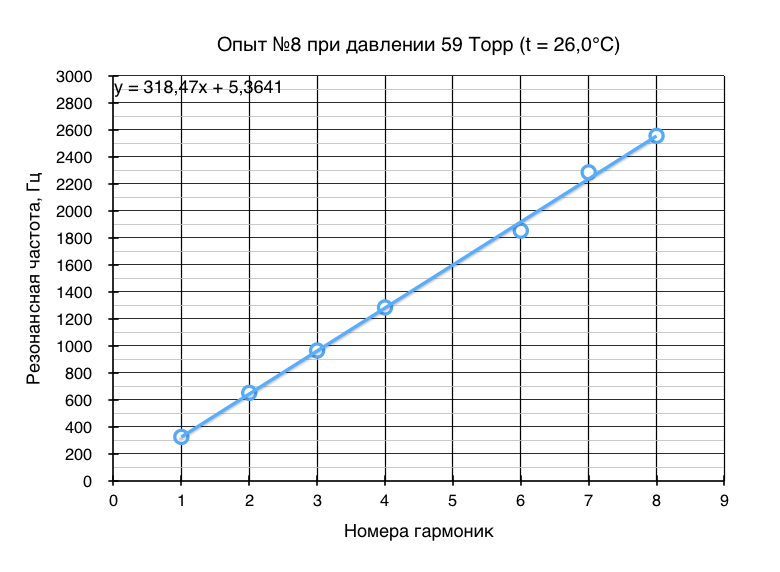
\includegraphics[width=70mm]{gr8.png}
		\hfill
		%\caption{Опыт №1}
		\label{gr8}
		\hfill
		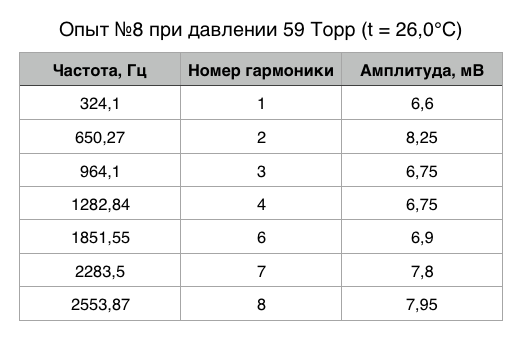
\includegraphics[width=70mm]{t8.png}
		\hfill
		%caption{Опыт №1}
		\label{t8}
	\end{multicols}
\end{figure}
\clearpage
\setcounter{equation}{0}
\section{Вывод теоретической модели}
Скорость звука в газе определяется по формуле
\begin{equation}
	c = \sqrt{\left ( \frac{\partial P}{\partial \rho}\right )_S}
\end{equation}

\begin{equation}
	\left ( \frac{\partial P}{\partial \rho}\right )_S = - \frac{\left ( \frac{\partial S}{\partial \rho}\right )_P}{\left ( \frac{\partial S}{\partial P}\right )_\rho} 
\end{equation}

Для одного моля $V = \frac{m}{\rho} = \frac{\mu \nu}{\rho} = \frac{\mu}{\rho}$

\begin{equation}
	\left ( \frac{\partial V}{\partial \rho}\right )_P = - \frac{\mu}{\rho^2}
\end{equation}


\begin{equation}
	\left ( \frac{\partial P}{\partial \rho}\right )_S = - \,  \frac{\left ( \frac{\partial S}{\partial \rho}\right )_P}{\left ( \frac{\partial S}{\partial P}\right )_\rho} = - \, \frac{\left ( \frac{\partial V}{\partial \rho}\right )_P \left ( \frac{\partial S}{\partial V}\right )_P}{\left ( \frac{\partial S}{\partial P}\right )_V} = \frac{\mu}{\rho^2} \frac{T \left ( \frac{\partial S}{\partial V}\right )_P}{T \left ( \frac{\partial S}{\partial P}\right )_V}
\end{equation}

Используя соотношения
\begin{equation}
	\left ( \frac{\partial S}{\partial V}\right )_P =  \left ( \frac{\partial T}{\partial V}\right )_P \left ( \frac{\partial S}{\partial T}\right )_P
\end{equation}
\begin{equation}
	\left ( \frac{\partial S}{\partial P}\right )_V = \left ( \frac{\partial S}{\partial T}\right )_V \left ( \frac{\partial T}{\partial P}\right )_V
\end{equation}

\begin{equation}
	\left ( \frac{\partial S}{\partial T}\right )_P = \frac{C_P}{T}
\end{equation}
\begin{equation}
	\left ( \frac{\partial S}{\partial T}\right )_V = \frac{C_V}{T}
\end{equation}

Итого получаем
\begin{equation}
	\left ( \frac{\partial P}{\partial \rho}\right )_S = \frac{C_P}{C_V} \frac{\mu}{\rho^2}\frac{\left ( \frac{\partial T}{\partial V}\right )_P}{\left ( \frac{\partial T}{\partial P}\right )_V}
\end{equation}

Найдём $\left ( \frac{\partial T}{\partial V}\right )_P$ и $\left ( \frac{\partial T}{\partial P}\right )_V$

Исследуем модель газа Ван-дер-Ваальса:
\begin{equation}
	RT = \left(P + \frac{a}{V^2}\right)(V - b)
\end{equation}

\begin{equation}
	\left ( \frac{\partial T}{\partial V}\right )_P = \frac{1}{R} \left(P - \frac{a}{V^2} + \frac{2ab}{V^3}\right) 
\end{equation}

\begin{equation}
	\left ( \frac{\partial T}{\partial P}\right )_V = \frac{V - b}{R}
\end{equation}

\begin{equation}
	\left ( \frac{\partial T}{\partial V}\right )_P = \frac{P - \frac{a}{V^2} + \frac{2ab}{V^3}}{R}
\end{equation}

Далее найдём соотношение $\frac{C_P}{C_V}$
\begin{equation}
	\frac{C_P}{C_V} = \frac{\left ( \frac{\delta Q}{\partial T}\right )_P}{\left ( \frac{\delta Q}{\partial T}\right )_V} = \frac{\left ( \frac{\partial U}{\partial T}\right )_P + P\left ( \frac{\partial V}{\partial T}\right )_P}{\left ( \frac{\partial U}{\partial T}\right )_V}
\end{equation}

\begin{equation}
	C_V = \frac{i}{2}R
\end{equation}

\begin{equation}
	\left ( \frac{\partial V}{\partial T}\right )_P = \frac{1}{\left ( \frac{\partial T}{\partial V}\right )_P} = \frac{R}{P - \frac{a}{V^2} + \frac{2ab}{V^3}} \approx \frac{R}{P - \frac{a}{V^2}} \approx \frac{R}{P}\left(1 + \frac{a}{PV^2}\right)
\end{equation}

\begin{equation}
	U = \frac{i}{2}RT - \frac{a}{V(T)}
\end{equation}

\begin{equation}
	\left ( \frac{\partial U}{\partial T}\right )_P = \frac{a}{V^2}
\end{equation}

\begin{equation}
	dU = \frac{i}{2}RdT + \frac{a}{V^2}dV
\end{equation}

\begin{equation}
	\left ( \frac{\partial U}{\partial T}\right )_P = \frac{i}{2}R + \frac{a}{V^2}\left ( \frac{\partial V}{\partial T}\right )_P
\end{equation}
Подставим (16)
\begin{equation}
	\left ( \frac{\partial U}{\partial T}\right )_P = \frac{i}{2}R + \frac{a}{V^2}\frac{R}{P}\left(1 + \frac{1}{PV^2}\right)
\end{equation}

Получаем
\begin{equation}
	C_P = \frac{i}{2}R + R\left(1 + \frac{a}{PV^2}\right)^2 = \frac{i+2}{2}R + \frac{2aR}{PV^2}
\end{equation}

Тогда 
\begin{equation}
	\frac{C_P}{C_V} = \frac{\frac{i+2}{2}R + \frac{2aR}{PV^2}}{\frac{i}{2}R} = \gamma_0 + \frac{4aP}{iR^2T^2}
\end{equation}

Окончательно получаем 
\begin{equation}
	c = \sqrt{\left ( \frac{\partial P}{\partial \rho}\right )_S} = \sqrt{\left(\gamma_0 + \frac{4aP}{iR^2T^2}\right)\frac{\mu}{\rho^2}\frac{P - \frac{a}{V^2} + \frac{2ab}{V^3}}{V - b}}
\end{equation}

Итого зависимость скорости звука от давления:
\begin{equation}
	c = c_0 \left ( 1 + \frac{2aP}{iRT\mu c^2_0} \right )\left [ 1 + \frac{P}{2RT} \left ( b - \frac{a}{RT} + \frac{2Pab}{(RT)^2} \right ) \right ],
\end{equation}
где $c_0$ - скорость звука по формуле $c = \sqrt{\gamma \frac{RT}{\mu}}$ при определённой фиксированной температуре, a и b - коэффициенты Ван-дер-Ваальса, i - число степеней свободы газа.

На сайте tehtab.ru приведен экспериментальный график зависимости скорости звука в воздухе при температуре 20$^{\circ} C$ от давления при больших давлениях. Построим график такой же зависимости по выведенной нами формуле.
\begin{figure}[h]
	\begin{multicols}{2}
		\hfill
		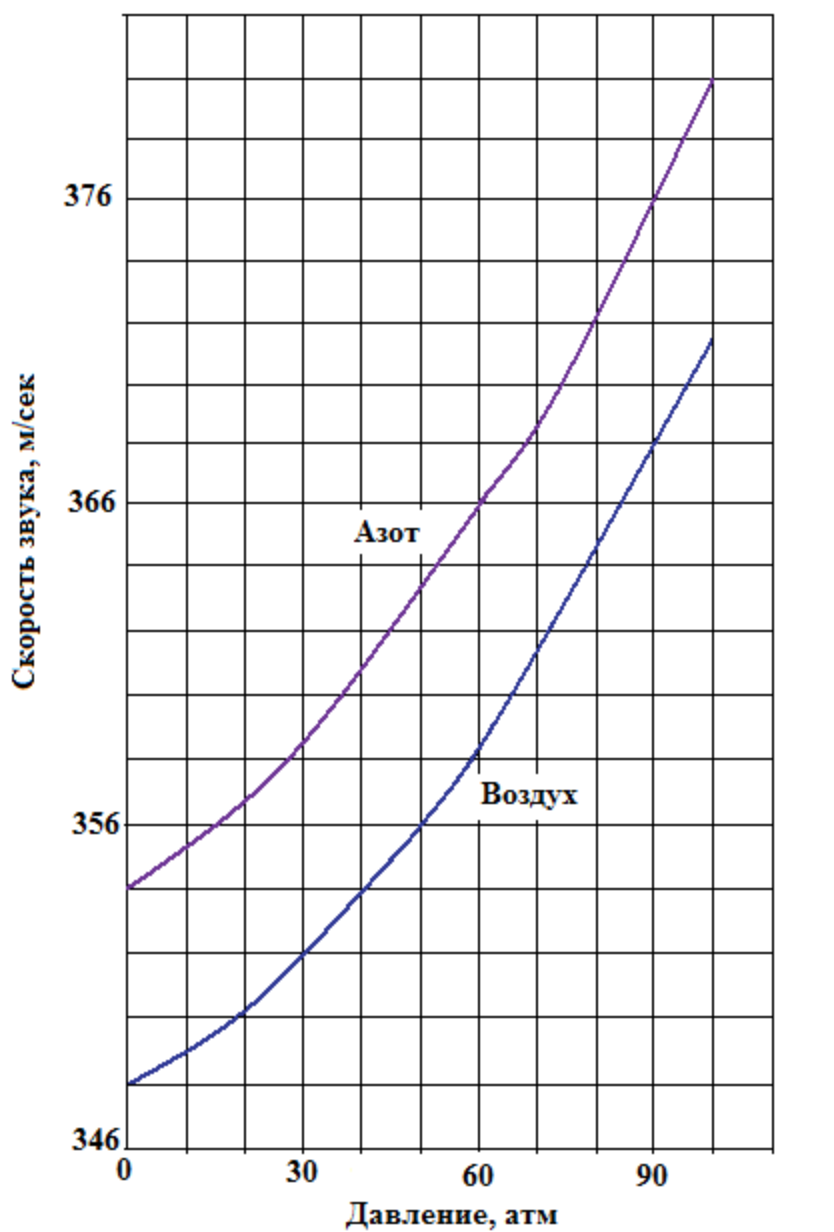
\includegraphics[width=55mm]{gr_tehtab.png}
		\hfill
		\caption{Экспериментальная зависимость}
		\label{gr_tehtab}
		\hfill
		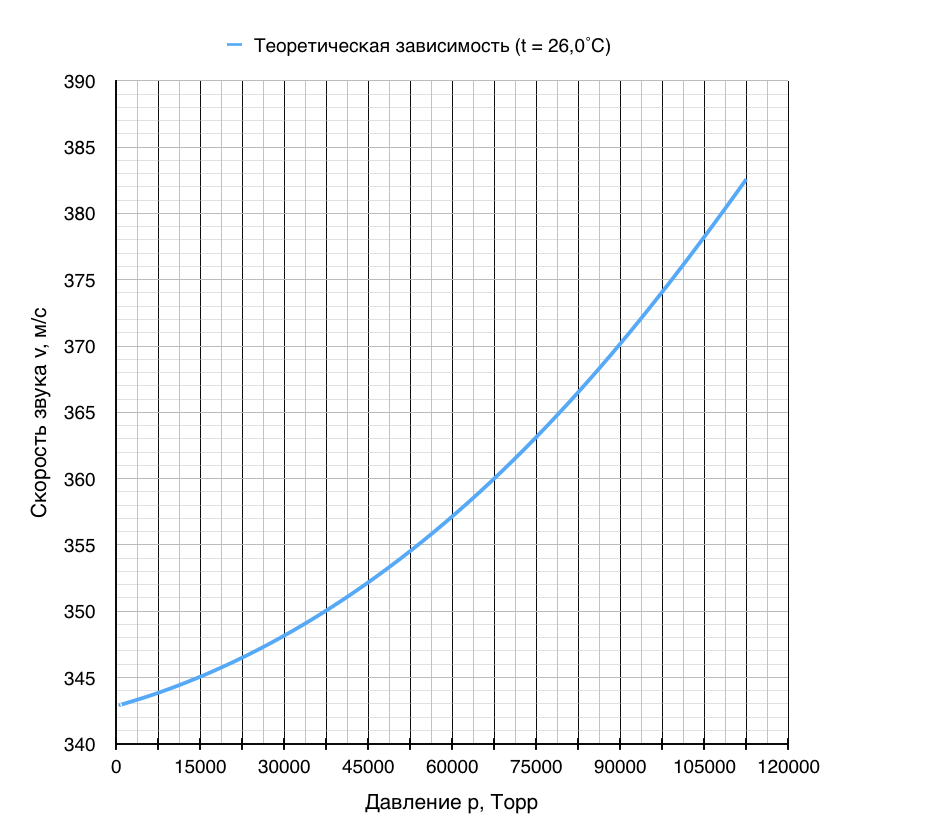
\includegraphics[width=90mm]{gr_ThLong.png}
		\hfill
		\caption{Предложенная теоретическая модель}
		\label{gr_ThLong}
	\end{multicols}
\end{figure}

Мы видим, что совпадает не только характер зависимости ($v \sim P^3 $), но и отдельные значения скорости звука при давлениях в несколько десятков атмосфер. Значит, предложенная нами зависимость применима в рабочем диапозоне давлений. 

\end{document}